\chapter{Testing and Result}\label{ch:testing}

\section{Introduction}\label{sec:testingIntroduction}

This chapter provides an overview of the testing scenarios associated with the \textbf{Collective} mobile journaling application. The importance of testing in the software development life cycle is paramount, as it ensures that the system operates reliably and meets user requirements. The primary goal of testing is to identify and resolve technical issues and bugs, ensuring the system functions correctly and aligns with the specified requirements outlined in Chapter~\ref{ch:methodology}.

Testing the Collective mobile journaling application involves evaluating the system's various functionalities including journal entry creation, user authentication, data storage and synchronization, AI-powered insights, and offline capabilities. Due to the complexity of the mobile application and the numerous possible input and output combinations across different Android devices, it is impractical to test every possible scenario. However, thorough testing aims to cover as many scenarios as possible to ensure robustness and reliability.

The chapter emphasizes four critical testing methodologies: \textbf{Integration Testing} to verify component interaction, \textbf{System Testing} to validate overall functionality, \textbf{User Acceptance Testing} with test cases specified in individual tables, and \textbf{Usability Testing} conducted through structured feedback gathering with respondents as testers. By adhering to these testing standards, the chapter aims to demonstrate how the Collective mobile journaling application meets quality standards and fulfills user requirements.

\section{Test Objective}\label{sec:testObjective}

The test plan focuses on identifying and documenting as many bugs as possible to enhance the system's reliability. The \textbf{Collective} mobile journaling application underwent extensive testing through four testing phases: Integration Testing to verify component interactions, System Testing to validate complete functionality, User Acceptance Testing with test cases documented in individual tables, and Usability Testing conducted through structured feedback gathering with respondents as testers.

The application testing focused on crucial operations such as journal entry creation, editing, deletion, user authentication, data synchronization, and AI-powered insights generation. The user interface has been carefully crafted to ensure ease of use, facilitating smooth navigation throughout the journaling experience. Throughout the development process, emphasis has been placed on performance and usability to ensure a seamless journaling experience.

\section{Test Process}\label{sec:testProcess}

Figure~\ref{fig:test-process} illustrates the Test Process approach as follows:

\textbf{i. 60\% development progress:} At this stage, the majority of core features are implemented including Flutter framework setup, Firebase authentication, journal entry creation, AI-powered insights integration, and basic offline functionality. This milestone provides sufficient functionality for initial integration testing.

\textbf{ii. Integration Testing:} With core components developed, integration testing begins to verify that different modules work together seamlessly. This includes testing the integration between Firebase authentication, local database storage with Sembast, AI service connectivity with DeepSeek API, and user interface elements to ensure effective communication between components.

\textbf{iii. 80\% development progress:} Following successful integration testing, development continues with advanced features such as enhanced offline synchronization, media attachment capabilities, analytics dashboard, and bookmark management functionality.

\textbf{iv. System Testing:} At this development milestone, comprehensive system testing evaluates the entire Collective mobile journaling application to verify that all specifications and requirements are met. Both functional and non-functional aspects, such as performance, offline functionality, and data synchronization, are thoroughly tested across different Android devices.

\textbf{v. 95\% development progress:} With system testing completed and major issues resolved, the application reaches near-completion status with all critical features implemented and tested, ready for final user validation.

\textbf{vi. User Acceptance Testing:} At this advanced stage, the system undergoes comprehensive test case validation covering all functional requirements. Individual test cases are documented in dedicated tables to ensure systematic coverage of all system features and user scenarios.

\textbf{vii. Usability Testing:} In this final phase, the nearly complete system undergoes usability evaluation through structured feedback gathering with respondents as testers. The Collective mobile journaling application must demonstrate ease of use and user satisfaction to validate its core objective of providing a simplified, distraction-free digital journaling experience.

\begin{figure}[H]
\centering
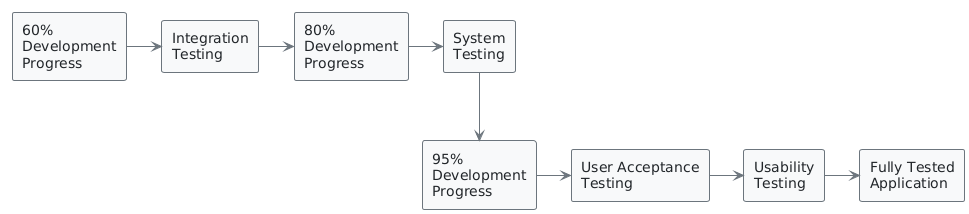
\includegraphics[width=0.8\textwidth]{files/imgs/test_process_flow.png}
\caption{Test Process Flow for Collective Mobile Journaling Application}
\label{fig:test-process}
\end{figure}

\subsection{Risk and Contingencies}\label{sec:riskContingencies}

Several risk-related issues need to be addressed with contingency during testing as they could lead to major troublesome problems that will affect testing development. There are project and product risks; for product risks, they will be specified in risk-based testing sections, while here are the project risks for the Collective mobile journaling application testing:

\begin{table}[H]
\centering
\caption{Risks and Contingencies for Collective Mobile Journaling Application Testing}
\label{tab:risks-contingencies}
\begin{tabular}{|p{1cm}|p{4cm}|p{3cm}|p{6cm}|}
\hline
\textbf{ID NO} & \textbf{Project Risks} & \textbf{Impact} & \textbf{Contingencies} \\
\hline
1 & Unavailability of Android test devices & Unable to run mobile tests and delay testing schedule & Proper planning and preparing checklist to ensure all Android devices are available. If event occurs, use emulators or request additional devices from colleagues. \\
\hline
2 & Firebase backend service downtime & Unable to test authentication, cloud sync, and data storage features & Implement local testing environment with mock Firebase services. Schedule tests during stable service hours and have backup testing scenarios. \\
\hline
3 & DeepSeek API rate limiting or service unavailability & Cannot test AI-powered insights and analysis features & Implement mock AI responses for testing. Cache previous API responses for test scenarios. Consider alternative AI service testing. \\
\hline
4 & Internet connectivity issues & Unable to test online features, cloud synchronization, and API integrations & Focus on offline functionality testing first. Use mobile hotspot as backup connection. Prepare test scenarios for both online and offline modes. \\
\hline
5 & Time and resource limitations & Not enough time to complete comprehensive testing across all features & Prioritize critical path testing and core functionalities. Eliminate low-priority test cases. Focus on integration and system testing for essential features. \\
\hline
6 & Large number of defects found during integration testing & Unable to proceed with system and user acceptance testing & Implement defect triage system. Fix critical defects first. Parallel testing and development approach for non-blocking issues. \\
\hline
7 & Lack of real user data for testing & Test scenarios may not reflect actual usage patterns & Generate realistic test data based on user research. Recruit beta testers for realistic data creation. Use anonymized sample journal entries. \\
\hline
8 & Changes in Flutter framework or Firebase SDK versions & Compatibility issues affecting test environment stability & Maintain version control and testing on multiple framework versions. Keep rollback options available. Document version-specific test procedures. \\
\hline
9 & Insufficient knowledge of mobile testing tools and methodologies & Delayed testing process and potential test inaccuracy & Consult with mobile development experts and supervisor. Conduct training on Flutter testing frameworks. Research mobile testing best practices. \\
\hline
10 & User recruitment challenges for usability testing & Limited or biased feedback for user acceptance and usability evaluation & Expand recruitment channels including social media and university networks. Offer incentives for participation. Use remote testing tools if needed. \\
\hline
\end{tabular}
\end{table}

\subsection{Test Environment}\label{sec:testEnvironment}

This section of the chapter provides an overview of the necessary resources that are essential for creating the test environment and conducting the testing process for the Collective mobile journaling application. These resources encompass hardware components, software applications, and any other specific requirements that are necessary for mobile application testing purposes.

\begin{table}[H]
\centering
\caption{Hardware Requirements for Collective Mobile App Testing}
\label{tab:hardware-test-requirements}
\begin{tabular}{|p{6cm}|p{8cm}|}
\hline
\textbf{Hardware Requirements} & \textbf{Specifications} \\
\hline
Operating System & Windows 10/11 or macOS (for development environment) \\
\hline
Installed Memory (RAM) & 16.00 GB or above (recommended for Flutter development and Android emulation) \\
\hline
CPU & Intel Core i7 or AMD Ryzen 7 or above \\
\hline
Processor Speed & 2.40 GHz or above \\
\hline
Storage & 256 GB SSD or above (for fast compilation and emulator performance) \\
\hline
Android Test Devices & Multiple Android devices with API levels 21-34 (Android 5.0 to Android 14) \\
\hline
Network Connection & Stable internet connection for Firebase testing and DeepSeek API integration \\
\hline
\end{tabular}
\end{table}

\begin{table}[H]
\centering
\caption{Software Requirements for Collective Mobile App Testing}
\label{tab:software-requirements}
\begin{tabular}{|p{1cm}|p{4cm}|p{9cm}|}
\hline
\textbf{NO} & \textbf{SOFTWARE} & \textbf{DESCRIPTION} \\
\hline
1 & Flutter SDK & Flutter is Google's UI toolkit for building natively compiled applications for mobile from a single codebase. Essential for developing and testing the Collective mobile journaling application with Dart programming language. \\
\hline
2 & Android Studio & Android Studio is the official integrated development environment (IDE) for Android development. Provides Android emulators, debugging tools, and device testing capabilities essential for mobile application testing. \\
\hline
3 & Visual Studio Code & Visual Studio Code is a lightweight code editor with excellent Flutter and Dart extensions. Used for code development, debugging, and integration with Firebase services for the Collective application. \\
\hline
4 & Firebase Console & Firebase Console is a web-based platform for managing Firebase services including Authentication, Firestore database, and Storage. Essential for testing cloud-based features and monitoring application performance. \\
\hline
5 & Git and GitHub & Version control system for tracking code changes and collaborative development. Essential for maintaining test code versions and coordinating testing across different development stages. \\
\hline
6 & Postman & API testing tool used for testing DeepSeek API integration, Firebase REST APIs, and other web service endpoints used by the Collective mobile application. \\
\hline
7 & Firebase CLI & Command-line interface for Firebase services, enabling local testing, deployment, and management of Firebase functions and hosting for testing purposes. \\
\hline
8 & Chrome DevTools & Web debugging tools for testing web views and debugging network requests within the mobile application, particularly useful for API testing and performance monitoring. \\
\hline
9 & Figma & Cloud-based design tool for accessing and validating UI/UX design specifications during testing. Ensures the implemented application matches the intended design requirements. \\
\hline
10 & Microsoft Office & Productivity suite for creating test documentation, test case reports, user acceptance testing forms, and usability testing questionnaires for the Collective mobile application. \\
\hline
\end{tabular}
\end{table}

\begin{table}[H]
\centering
\caption{Testing Group for Collective Mobile Journaling Application}
\label{tab:testing-group}
\begin{tabular}{|p{6cm}|p{8cm}|}
\hline
\textbf{Test Sequence} & \textbf{Tester} \\
\hline
Registration & WAN AMINNUR RASHEED \\
\hline
Login Authentication & WAN AMINNUR RASHEED \\
\hline
Journal Entry Creation & WAN AMINNUR RASHEED \\
\hline
Journal Entry Editing & WAN AMINNUR RASHEED \\
\hline
Journal Entry Deletion & WAN AMINNUR RASHEED \\
\hline
AI Insights Generation & WAN AMINNUR RASHEED \\
\hline
Image Attachment & WAN AMINNUR RASHEED \\
\hline
Bookmark Management & WAN AMINNUR RASHEED \\
\hline
Offline Functionality & WAN AMINNUR RASHEED \\
\hline
Data Synchronization & WAN AMINNUR RASHEED \\
\hline
Search Functionality & WAN AMINNUR RASHEED \\
\hline
Analytics Dashboard & WAN AMINNUR RASHEED \\
\hline
User Profile Management & WAN AMINNUR RASHEED \\
\hline
Social Authentication (Google) & WAN AMINNUR RASHEED \\
\hline
Social Authentication (Twitter/X) & WAN AMINNUR RASHEED \\
\hline
Theme Switching & WAN AMINNUR RASHEED \\
\hline
Performance Testing & WAN AMINNUR RASHEED \\
\hline
Security Testing & WAN AMINNUR RASHEED \\
\hline
Usability Testing & WAN AMINNUR RASHEED \\
\hline
Integration Testing & WAN AMINNUR RASHEED \\
\hline
\end{tabular}
\end{table}

\section{Testing Plan and Testing Approach}\label{sec:testingPlan}

In software development, testing is crucial to ensure the system meets client requirements and functions correctly. This section outlines the tests conducted for the Collective mobile journaling application, including unit testing, integration testing, system testing, and user acceptance testing.

\subsection{Testing Approach}\label{sec:testingApproach}

In this testing planning, there are two types of test approaches that are used:

\textbf{i. Preventive Approach:} A quick design check approach test was employed to swiftly review the design. At the outset of development, user requirements were gathered, identified, and scrutinized to eliminate any ambiguities in the system requirements. This approach ensures that potential issues are identified and resolved during the design phase before implementation begins.

\textbf{ii. Reactive Approach:} After programming, a concept test is conducted to assess the system's functionality. This test involves executing the code to ensure that the Collective mobile journaling application functions correctly across different Android devices and usage scenarios.

\subsection{Unit Testing}\label{sec:unitTesting}

Unit testing for the Collective mobile journaling application will be split into two phases. The first phase will encompass the initial 60\% of module development, addressing core features such as user authentication, journal entry creation, local database storage, and basic AI integration. The second phase will cover the remaining 40\% of module development, encompassing advanced features including offline synchronization, analytics dashboard, bookmark management, and enhanced AI insights functionality.

\subsection{Integration Testing}\label{sec:integrationTesting}

Integration testing assesses the integration of modules with one another within the Collective mobile journaling application. This involves checking modules such as Firebase authentication for integration with local Sembast database storage, ensuring they successfully link with cloud services and AI APIs without errors. The testing reviews all components to ensure seamless integration between the Flutter frontend, Firebase backend services, DeepSeek AI API, and local storage systems. Key integration points include user authentication flow, data synchronization between local and cloud storage, AI service connectivity, and image attachment processing.

\subsection{System Testing}\label{sec:systemTesting}

System testing aims to uncover defects that are only evident when testing the entire integrated Collective mobile journaling application or a significant portion of it. While it typically addresses performance, security, and validation concerns, this project primarily focuses on functional validation, efficiency, and load testing across different Android devices. The testing will ensure each component behaves as intended, including verifying that user interface elements respond correctly to touch interactions, data entry functions work seamlessly, and AI-powered insights generate accurately. Additionally, it will assess the interaction between the mobile interface and both local and cloud databases, ensuring data processing yields the expected outcomes, synchronization works correctly, and retrieved information is accurate across online and offline scenarios.

\subsection{User Acceptance Testing}\label{sec:userAcceptanceTesting}

User acceptance testing for the Collective mobile journaling application involves comprehensive validation with target users to ensure the application meets their journaling needs and expectations. The primary objective is to verify that the application successfully provides a simplified, distraction-free digital journaling experience that bridges traditional and digital journaling approaches. The testing focuses on real-world usage scenarios, enabling users to verify that the application meets their requirements for daily journaling, AI-powered insights, and seamless user experience.

Test cases are developed from user acceptance criteria and business use cases to thoroughly evaluate and validate the application before final acceptance and deployment. They focus on real-life scenarios such as daily journal entry creation, mood tracking, image attachment, AI insights generation, and offline usage patterns. The application has been designed to meet typical journaling requirements with potential for further enhancements based on user feedback. The details of the test cases are shown in tables~\ref{tab:test-case-login} through~\ref{tab:test-case-usability}.

\begin{table}[H]
\centering
\caption{Test Case Login Authentication}
\label{tab:test-case-login}
\begin{tabular}{|p{4cm}|p{10cm}|}
\hline
\textbf{Test Type} & Black box Testing – Functional Testing \\
\hline
\textbf{Test Case ID} & TC01 \\
\hline
\textbf{Test Case Name} & Login Authentication \\
\hline
\textbf{Test Case Details} & To test the Login module to verify user authentication functionality for the Collective mobile journaling application. Users login to gain access to journaling features and personal data. It will authenticate users and redirect to the main journal interface. \\
\hline
\textbf{Tested By} & WAN AMINNUR RASHEED \\
\hline
\textbf{Item(s) that will be tested} & Email/password login, Google authentication, Twitter/X authentication \\
\hline
\multicolumn{2}{|l|}{\textbf{Specifications}} \\
\hline
\textbf{Input Step(s)} & \textbf{Expected Output} \\
\hline
Users fill the login details (email, password) or select social login & 1. Display login form with email/password fields and social login options. \newline 2. Display error notification if credentials are invalid. \newline 3. If credentials are valid, authenticate user and redirect to main journal interface. \newline 4. For social login, redirect to respective OAuth provider and return with authentication. \\
\hline
\multicolumn{2}{|l|}{\textbf{Procedural Steps}} \\
\hline
\multicolumn{2}{|p{14cm}|}{1. Navigate to login screen. \newline 2. Users select authentication method (email/password, Google, or Twitter/X). \newline 3. Users fill up the login form or complete social authentication. \newline 4. Users tap the login button or confirm social login. \newline 5. If invalid credentials, display error and return to step 2. \newline 6. User successfully logs into the Collective application and accesses journal interface.} \\
\hline
\end{tabular}
\end{table}

\begin{table}[H]
\centering
\caption{Test Case Registration}
\label{tab:test-case-registration}
\begin{tabular}{|p{4cm}|p{10cm}|}
\hline
\textbf{Test Type} & Black box Testing – Functional Testing \\
\hline
\textbf{Test Case ID} & TC02 \\
\hline
\textbf{Test Case Name} & User Registration \\
\hline
\textbf{Test Case Details} & To test the registration module for new users to create accounts in the Collective mobile journaling application. Users provide necessary information to create their journaling account. \\
\hline
\textbf{Tested By} & WAN AMINNUR RASHEED \\
\hline
\textbf{Item(s) that will be tested} & Email registration, password validation, account creation, Firebase user creation \\
\hline
\multicolumn{2}{|l|}{\textbf{Specifications}} \\
\hline
\textbf{Input Step(s)} & \textbf{Expected Output} \\
\hline
Users fill registration form (email, password, confirm password) & 1. Display registration form with required fields. \newline 2. Validate email format and password strength. \newline 3. Display error if passwords don't match or email exists. \newline 4. Create user account and redirect to journal interface. \\
\hline
\multicolumn{2}{|l|}{\textbf{Procedural Steps}} \\
\hline
\multicolumn{2}{|p{14cm}|}{1. Navigate to registration screen. \newline 2. Users fill in email and password fields. \newline 3. Users confirm password in confirmation field. \newline 4. Users tap register button. \newline 5. If validation fails, display error and return to step 2. \newline 6. User account successfully created and user is logged in.} \\
\hline
\end{tabular}
\end{table}

\begin{table}[H]
\centering
\caption{Test Case Journal Entry Creation}
\label{tab:test-case-journal-creation}
\begin{tabular}{|p{4cm}|p{10cm}|}
\hline
\textbf{Test Type} & Black box Testing – Functional Testing \\
\hline
\textbf{Test Case ID} & TC03 \\
\hline
\textbf{Test Case Name} & Journal Entry Creation \\
\hline
\textbf{Test Case Details} & To test the core functionality of creating new journal entries with text content, mood selection, and optional image attachments. \\
\hline
\textbf{Tested By} & WAN AMINNUR RASHEED \\
\hline
\textbf{Item(s) that will be tested} & Text input, mood selection, image attachment, save functionality, local storage \\
\hline
\multicolumn{2}{|l|}{\textbf{Specifications}} \\
\hline
\textbf{Input Step(s)} & \textbf{Expected Output} \\
\hline
Users write journal text, select mood, optionally attach image & 1. Display clean writing interface. \newline 2. Accept text input and mood selection. \newline 3. Allow image attachment from gallery or camera. \newline 4. Save entry to local database and sync to cloud. \\
\hline
\multicolumn{2}{|l|}{\textbf{Procedural Steps}} \\
\hline
\multicolumn{2}{|p{14cm}|}{1. Navigate to new entry screen. \newline 2. Users type journal content in text field. \newline 3. Users select mood from available options. \newline 4. Users optionally attach image via camera or gallery. \newline 5. Users tap save button. \newline 6. Entry is saved locally and queued for cloud sync.} \\
\hline
\end{tabular}
\end{table}

\begin{table}[H]
\centering
\caption{Test Case Journal Entry Editing}
\label{tab:test-case-journal-editing}
\begin{tabular}{|p{4cm}|p{10cm}|}
\hline
\textbf{Test Type} & Black box Testing – Functional Testing \\
\hline
\textbf{Test Case ID} & TC04 \\
\hline
\textbf{Test Case Name} & Journal Entry Editing \\
\hline
\textbf{Test Case Details} & To test the ability to edit existing journal entries, modify content, mood, and manage image attachments. \\
\hline
\textbf{Tested By} & WAN AMINNUR RASHEED \\
\hline
\textbf{Item(s) that will be tested} & Edit text content, mood modification, image replacement, update functionality \\
\hline
\multicolumn{2}{|l|}{\textbf{Specifications}} \\
\hline
\textbf{Input Step(s)} & \textbf{Expected Output} \\
\hline
Users modify existing entry content, mood, or images & 1. Load existing entry data into edit form. \newline 2. Allow modification of text, mood, and images. \newline 3. Preserve original data if user cancels. \newline 4. Update entry in local and cloud storage. \\
\hline
\multicolumn{2}{|l|}{\textbf{Procedural Steps}} \\
\hline
\multicolumn{2}{|p{14cm}|}{1. Select existing journal entry from list. \newline 2. Tap edit button to enter edit mode. \newline 3. Modify text content, mood, or images as needed. \newline 4. Tap save to confirm changes or cancel to discard. \newline 5. Updated entry is saved and synchronized.} \\
\hline
\end{tabular}
\end{table}

\begin{table}[H]
\centering
\caption{Test Case AI Insights Generation}
\label{tab:test-case-ai-insights}
\begin{tabular}{|p{4cm}|p{10cm}|}
\hline
\textbf{Test Type} & Black box Testing – Functional Testing \\
\hline
\textbf{Test Case ID} & TC05 \\
\hline
\textbf{Test Case Name} & AI Insights Generation \\
\hline
\textbf{Test Case Details} & To test the AI-powered analysis functionality that generates insights, patterns, and suggestions based on journal entries using DeepSeek API. \\
\hline
\textbf{Tested By} & WAN AMINNUR RASHEED \\
\hline
\textbf{Item(s) that will be tested} & DeepSeek API integration, insight generation, pattern analysis, recommendation display \\
\hline
\multicolumn{2}{|l|}{\textbf{Specifications}} \\
\hline
\textbf{Input Step(s)} & \textbf{Expected Output} \\
\hline
Users request AI insights for journal entries & 1. Analyze journal content using DeepSeek API. \newline 2. Generate meaningful insights and patterns. \newline 3. Display insights in user-friendly format. \newline 4. Handle API failures gracefully with fallback messages. \\
\hline
\multicolumn{2}{|l|}{\textbf{Procedural Steps}} \\
\hline
\multicolumn{2}{|p{14cm}|}{1. Navigate to insights or analytics section. \newline 2. Select entries or time period for analysis. \newline 3. Tap generate insights button. \newline 4. System processes entries through AI service. \newline 5. Display generated insights, patterns, and recommendations.} \\
\hline
\end{tabular}
\end{table}

\begin{table}[H]
\centering
\caption{Test Case Offline Functionality}
\label{tab:test-case-offline}
\begin{tabular}{|p{4cm}|p{10cm}|}
\hline
\textbf{Test Type} & Black box Testing – Functional Testing \\
\hline
\textbf{Test Case ID} & TC06 \\
\hline
\textbf{Test Case Name} & Offline Functionality \\
\hline
\textbf{Test Case Details} & To test the application's ability to function without internet connectivity, including creating, editing, and viewing journal entries offline. \\
\hline
\textbf{Tested By} & WAN AMINNUR RASHEED \\
\hline
\textbf{Item(s) that will be tested} & Offline data storage, local database operations, sync queue management, connectivity detection \\
\hline
\multicolumn{2}{|l|}{\textbf{Specifications}} \\
\hline
\textbf{Input Step(s)} & \textbf{Expected Output} \\
\hline
Users perform journaling activities without internet connection & 1. Detect offline status and display indicator. \newline 2. Allow full functionality using local database. \newline 3. Queue changes for synchronization when online. \newline 4. Maintain data integrity across offline/online transitions. \\
\hline
\multicolumn{2}{|l|}{\textbf{Procedural Steps}} \\
\hline
\multicolumn{2}{|p{14cm}|}{1. Disable internet connectivity on device. \newline 2. Open Collective application. \newline 3. Create, edit, and view journal entries. \newline 4. Verify all functions work with local data. \newline 5. Re-enable connectivity and verify sync operation.} \\
\hline
\end{tabular}
\end{table}

\begin{table}[H]
\centering
\caption{Test Case Data Synchronization}
\label{tab:test-case-sync}
\begin{tabular}{|p{4cm}|p{10cm}|}
\hline
\textbf{Test Type} & Black box Testing – Functional Testing \\
\hline
\textbf{Test Case ID} & TC07 \\
\hline
\textbf{Test Case Name} & Data Synchronization \\
\hline
\textbf{Test Case Details} & To test the synchronization of journal entries between local storage and Firebase cloud storage, ensuring data consistency across devices. \\
\hline
\textbf{Tested By} & WAN AMINNUR RASHEED \\
\hline
\textbf{Item(s) that will be tested} & Firebase Firestore sync, conflict resolution, bidirectional sync, data integrity \\
\hline
\multicolumn{2}{|l|}{\textbf{Specifications}} \\
\hline
\textbf{Input Step(s)} & \textbf{Expected Output} \\
\hline
Users create/modify entries offline and come back online & 1. Detect connectivity restoration. \newline 2. Upload local changes to Firebase. \newline 3. Download remote changes to local storage. \newline 4. Resolve conflicts appropriately and maintain data integrity. \\
\hline
\multicolumn{2}{|l|}{\textbf{Procedural Steps}} \\
\hline
\multicolumn{2}{|p{14cm}|}{1. Create entries while offline. \newline 2. Restore internet connectivity. \newline 3. Observe automatic synchronization process. \newline 4. Verify entries appear in Firebase console. \newline 5. Test conflict resolution with simultaneous changes.} \\
\hline
\end{tabular}
\end{table}

\begin{table}[H]
\centering
\caption{Test Case Search Functionality}
\label{tab:test-case-search}
\begin{tabular}{|p{4cm}|p{10cm}|}
\hline
\textbf{Test Type} & Black box Testing – Functional Testing \\
\hline
\textbf{Test Case ID} & TC08 \\
\hline
\textbf{Test Case Name} & Search Functionality \\
\hline
\textbf{Test Case Details} & To test the search and filtering capabilities for finding specific journal entries based on content, date, mood, or tags. \\
\hline
\textbf{Tested By} & WAN AMINNUR RASHEED \\
\hline
\textbf{Item(s) that will be tested} & Text search, date filtering, mood filtering, tag search, search performance \\
\hline
\multicolumn{2}{|l|}{\textbf{Specifications}} \\
\hline
\textbf{Input Step(s)} & \textbf{Expected Output} \\
\hline
Users enter search terms or apply filters to find entries & 1. Display search interface with filter options. \newline 2. Process search queries efficiently. \newline 3. Return relevant results ranked by relevance. \newline 4. Handle empty results gracefully. \\
\hline
\multicolumn{2}{|l|}{\textbf{Procedural Steps}} \\
\hline
\multicolumn{2}{|p{14cm}|}{1. Navigate to search interface. \newline 2. Enter search terms or select filters (date, mood, tags). \newline 3. Tap search button or apply filters. \newline 4. Review search results. \newline 5. Tap on result to open specific entry.} \\
\hline
\end{tabular}
\end{table}

\begin{table}[H]
\centering
\caption{Test Case Bookmark Management}
\label{tab:test-case-bookmark}
\begin{tabular}{|p{4cm}|p{10cm}|}
\hline
\textbf{Test Type} & Black box Testing – Functional Testing \\
\hline
\textbf{Test Case ID} & TC09 \\
\hline
\textbf{Test Case Name} & Bookmark Management \\
\hline
\textbf{Test Case Details} & To test the ability to bookmark important journal entries for quick access and manage favorite entries collection. \\
\hline
\textbf{Tested By} & WAN AMINNUR RASHEED \\
\hline
\textbf{Item(s) that will be tested} & Add/remove bookmarks, bookmark persistence, favorites view, bookmark synchronization \\
\hline
\multicolumn{2}{|l|}{\textbf{Specifications}} \\
\hline
\textbf{Input Step(s)} & \textbf{Expected Output} \\
\hline
Users bookmark and manage favorite journal entries & 1. Allow bookmarking of entries with visual indicator. \newline 2. Provide dedicated favorites/bookmarks view. \newline 3. Persist bookmark status across sessions. \newline 4. Synchronize bookmarks across devices. \\
\hline
\multicolumn{2}{|l|}{\textbf{Procedural Steps}} \\
\hline
\multicolumn{2}{|p{14cm}|}{1. View journal entry and tap bookmark icon. \newline 2. Verify bookmark indicator changes state. \newline 3. Navigate to bookmarks/favorites section. \newline 4. Verify bookmarked entry appears in list. \newline 5. Test removing bookmark and verify removal.} \\
\hline
\end{tabular}
\end{table}

\begin{table}[H]
\centering
\caption{Test Case User Profile Management}
\label{tab:test-case-profile}
\begin{tabular}{|p{4cm}|p{10cm}|}
\hline
\textbf{Test Type} & Black box Testing – Functional Testing \\
\hline
\textbf{Test Case ID} & TC10 \\
\hline
\textbf{Test Case Name} & User Profile Management \\
\hline
\textbf{Test Case Details} & To test user profile creation, updates, and management including preferences, settings, and account information. \\
\hline
\textbf{Tested By} & WAN AMINNUR RASHEED \\
\hline
\textbf{Item(s) that will be tested} & Profile creation, information updates, preferences settings, account management \\
\hline
\multicolumn{2}{|l|}{\textbf{Specifications}} \\
\hline
\textbf{Input Step(s)} & \textbf{Expected Output} \\
\hline
Users access and modify profile information and settings & 1. Display current profile information. \newline 2. Allow editing of modifiable fields. \newline 3. Validate input data and save changes. \newline 4. Update profile across all app sections. \\
\hline
\multicolumn{2}{|l|}{\textbf{Procedural Steps}} \\
\hline
\multicolumn{2}{|p{14cm}|}{1. Navigate to profile/settings screen. \newline 2. View current profile information. \newline 3. Modify user preferences and settings. \newline 4. Save changes and verify updates. \newline 5. Test settings persistence across app sessions.} \\
\hline
\end{tabular}
\end{table}

\begin{table}[H]
\centering
\caption{Test Case Image Attachment}
\label{tab:test-case-image}
\begin{tabular}{|p{4cm}|p{10cm}|}
\hline
\textbf{Test Type} & Black box Testing – Functional Testing \\
\hline
\textbf{Test Case ID} & TC11 \\
\hline
\textbf{Test Case Name} & Image Attachment \\
\hline
\textbf{Test Case Details} & To test the functionality of attaching, viewing, and managing images within journal entries from camera or gallery sources. \\
\hline
\textbf{Tested By} & WAN AMINNUR RASHEED \\
\hline
\textbf{Item(s) that will be tested} & Camera capture, gallery selection, image compression, storage management, image display \\
\hline
\multicolumn{2}{|l|}{\textbf{Specifications}} \\
\hline
\textbf{Input Step(s)} & \textbf{Expected Output} \\
\hline
Users attach images from camera or gallery to journal entries & 1. Provide options for camera capture or gallery selection. \newline 2. Compress images appropriately for storage efficiency. \newline 3. Display attached images within journal entries. \newline 4. Store images locally and sync to Firebase Storage. \\
\hline
\multicolumn{2}{|l|}{\textbf{Procedural Steps}} \\
\hline
\multicolumn{2}{|p{14cm}|}{1. Create new journal entry or edit existing entry. \newline 2. Tap image attachment button. \newline 3. Select camera or gallery option. \newline 4. Capture photo or select from gallery. \newline 5. Confirm image attachment and save entry. \newline 6. Verify image appears in journal entry and syncs to cloud.} \\
\hline
\end{tabular}
\end{table}

\begin{table}[H]
\centering
\caption{Test Case Analytics Dashboard}
\label{tab:test-case-analytics}
\begin{tabular}{|p{4cm}|p{10cm}|}
\hline
\textbf{Test Type} & Black box Testing – Functional Testing \\
\hline
\textbf{Test Case ID} & TC12 \\
\hline
\textbf{Test Case Name} & Analytics Dashboard \\
\hline
\textbf{Test Case Details} & To test the analytics and insights dashboard that displays journaling patterns, mood trends, and writing statistics over time. \\
\hline
\textbf{Tested By} & WAN AMINNUR RASHEED \\
\hline
\textbf{Item(s) that will be tested} & Mood analytics, writing frequency charts, pattern visualization, statistical calculations \\
\hline
\multicolumn{2}{|l|}{\textbf{Specifications}} \\
\hline
\textbf{Input Step(s)} & \textbf{Expected Output} \\
\hline
Users view analytics dashboard to understand their journaling patterns & 1. Display comprehensive analytics interface. \newline 2. Show mood trends over selected time periods. \newline 3. Present writing frequency and word count statistics. \newline 4. Generate visual charts and insights. \\
\hline
\multicolumn{2}{|l|}{\textbf{Procedural Steps}} \\
\hline
\multicolumn{2}{|p{14cm}|}{1. Navigate to analytics or insights section. \newline 2. Select time period for analysis (week, month, year). \newline 3. View mood trend charts and patterns. \newline 4. Review writing frequency and statistics. \newline 5. Interact with charts for detailed information.} \\
\hline
\end{tabular}
\end{table}

\begin{table}[H]
\centering
\caption{Test Case Social Authentication}
\label{tab:test-case-social-auth}
\begin{tabular}{|p{4cm}|p{10cm}|}
\hline
\textbf{Test Type} & Black box Testing – Functional Testing \\
\hline
\textbf{Test Case ID} & TC13 \\
\hline
\textbf{Test Case Name} & Social Authentication \\
\hline
\textbf{Test Case Details} & To test Google and Twitter/X OAuth authentication integration for seamless user login and account creation. \\
\hline
\textbf{Tested By} & WAN AMINNUR RASHEED \\
\hline
\textbf{Item(s) that will be tested} & Google Sign-In, Twitter/X OAuth, account linking, profile data retrieval \\
\hline
\multicolumn{2}{|l|}{\textbf{Specifications}} \\
\hline
\textbf{Input Step(s)} & \textbf{Expected Output} \\
\hline
Users authenticate using Google or Twitter/X accounts & 1. Display social login options on authentication screen. \newline 2. Redirect to respective OAuth provider. \newline 3. Handle authentication callback and token exchange. \newline 4. Create or link user account and redirect to app. \\
\hline
\multicolumn{2}{|l|}{\textbf{Procedural Steps}} \\
\hline
\multicolumn{2}{|p{14cm}|}{1. Navigate to login screen. \newline 2. Select Google or Twitter/X authentication option. \newline 3. Complete OAuth flow with chosen provider. \newline 4. Authorize app permissions. \newline 5. Return to app with authenticated session. \newline 6. Verify profile data and app access.} \\
\hline
\end{tabular}
\end{table}

\begin{table}[H]
\centering
\caption{Test Case Theme Switching}
\label{tab:test-case-theme}
\begin{tabular}{|p{4cm}|p{10cm}|}
\hline
\textbf{Test Type} & Black box Testing – Functional Testing \\
\hline
\textbf{Test Case ID} & TC14 \\
\hline
\textbf{Test Case Name} & Theme Switching \\
\hline
\textbf{Test Case Details} & To test the light/dark theme switching functionality and system theme detection for optimal user experience. \\
\hline
\textbf{Tested By} & WAN AMINNUR RASHEED \\
\hline
\textbf{Item(s) that will be tested} & Light theme, dark theme, system theme detection, theme persistence \\
\hline
\multicolumn{2}{|l|}{\textbf{Specifications}} \\
\hline
\textbf{Input Step(s)} & \textbf{Expected Output} \\
\hline
Users switch between light, dark, and system themes & 1. Provide theme selection options in settings. \newline 2. Apply chosen theme across all app screens. \newline 3. Detect and follow system theme changes. \newline 4. Persist theme choice across app sessions. \\
\hline
\multicolumn{2}{|l|}{\textbf{Procedural Steps}} \\
\hline
\multicolumn{2}{|p{14cm}|}{1. Navigate to app settings or theme preferences. \newline 2. Select theme option (light, dark, or system). \newline 3. Verify theme applies immediately across app. \newline 4. Test system theme detection by changing device theme. \newline 5. Restart app and verify theme persistence.} \\
\hline
\end{tabular}
\end{table}

\begin{table}[H]
\centering
\caption{Test Case Performance Testing}
\label{tab:test-case-performance}
\begin{tabular}{|p{4cm}|p{10cm}|}
\hline
\textbf{Test Type} & Black box Testing – Performance Testing \\
\hline
\textbf{Test Case ID} & TC15 \\
\hline
\textbf{Test Case Name} & Performance Testing \\
\hline
\textbf{Test Case Details} & To test the application's performance under various load conditions including large datasets, memory usage, and response times. \\
\hline
\textbf{Tested By} & WAN AMINNUR RASHEED \\
\hline
\textbf{Item(s) that will be tested} & App startup time, data loading performance, memory usage, battery consumption, response times \\
\hline
\multicolumn{2}{|l|}{\textbf{Specifications}} \\
\hline
\textbf{Input Step(s)} & \textbf{Expected Output} \\
\hline
Test app performance with varying data loads and usage patterns & 1. Measure app startup and screen transition times. \newline 2. Monitor memory usage during intensive operations. \newline 3. Test performance with large journal datasets. \newline 4. Evaluate battery consumption during extended use. \\
\hline
\multicolumn{2}{|l|}{\textbf{Procedural Steps}} \\
\hline
\multicolumn{2}{|p{14cm}|}{1. Create large dataset of journal entries (1000+ entries). \newline 2. Measure app startup time and memory footprint. \newline 3. Test scrolling performance through large lists. \newline 4. Monitor CPU and battery usage during AI processing. \newline 5. Verify smooth animations and transitions.} \\
\hline
\end{tabular}
\end{table}

\begin{table}[H]
\centering
\caption{Test Case Security Testing}
\label{tab:test-case-security}
\begin{tabular}{|p{4cm}|p{10cm}|}
\hline
\textbf{Test Type} & Black box Testing – Security Testing \\
\hline
\textbf{Test Case ID} & TC16 \\
\hline
\textbf{Test Case Name} & Security Testing \\
\hline
\textbf{Test Case Details} & To test the security measures including data encryption, authentication security, and protection of sensitive user information. \\
\hline
\textbf{Tested By} & WAN AMINNUR RASHEED \\
\hline
\textbf{Item(s) that will be tested} & Data encryption, secure authentication, API security, local data protection \\
\hline
\multicolumn{2}{|l|}{\textbf{Specifications}} \\
\hline
\textbf{Input Step(s)} & \textbf{Expected Output} \\
\hline
Verify security measures protect user data and prevent unauthorized access & 1. Ensure journal data is encrypted in local storage. \newline 2. Verify secure transmission to Firebase. \newline 3. Test authentication token security. \newline 4. Validate API key protection and rate limiting. \\
\hline
\multicolumn{2}{|l|}{\textbf{Procedural Steps}} \\
\hline
\multicolumn{2}{|p{14cm}|}{1. Inspect local database encryption. \newline 2. Monitor network traffic for secure HTTPS connections. \newline 3. Test session timeout and re-authentication. \newline 4. Verify Firebase security rules prevent unauthorized access. \newline 5. Test API key security and rate limiting mechanisms.} \\
\hline
\end{tabular}
\end{table}

\begin{table}[H]
\centering
\caption{Test Case Usability Testing}
\label{tab:test-case-usability}
\begin{tabular}{|p{4cm}|p{10cm}|}
\hline
\textbf{Test Type} & Black box Testing – Usability Testing \\
\hline
\textbf{Test Case ID} & TC17 \\
\hline
\textbf{Test Case Name} & Usability Testing \\
\hline
\textbf{Test Case Details} & To evaluate the user experience, interface design, and ease of use through structured user testing sessions and feedback collection. \\
\hline
\textbf{Tested By} & WAN AMINNUR RASHEED \\
\hline
\textbf{Item(s) that will be tested} & User interface design, navigation flow, accessibility, user satisfaction, task completion rates \\
\hline
\multicolumn{2}{|l|}{\textbf{Specifications}} \\
\hline
\textbf{Input Step(s)} & \textbf{Expected Output} \\
\hline
Users complete typical journaling tasks while providing feedback & 1. Achieve high task completion rates (>85\%). \newline 2. Gather positive user satisfaction ratings. \newline 3. Identify and address usability issues. \newline 4. Validate intuitive interface design and navigation. \\
\hline
\multicolumn{2}{|l|}{\textbf{Procedural Steps}} \\
\hline
\multicolumn{2}{|p{14cm}|}{1. Recruit target users for testing sessions. \newline 2. Provide users with common journaling tasks. \newline 3. Observe user interactions and note difficulties. \newline 4. Collect feedback through surveys and interviews. \newline 5. Analyze results and implement improvements. \newline 6. Conduct follow-up testing to validate changes.} \\
\hline
\end{tabular}
\end{table}

\subsection{Usability Testing}\label{sec:usabilityTestingResults}

The primary goal of conducting a usability test is to assess the Collective mobile journaling application's ability to fulfill its intended purpose effectively. A questionnaire was used to gather feedback from respondents regarding the usability of the mobile application. Respondents were asked to evaluate the system based on their user experience, focusing on ease of use and digital journaling effectiveness. The target users for the questionnaire were UniKL students acting as beta testers. Prior to testing the system, participants were briefed on the application flow and provided with the APK file. They were informed that the testing aimed to assess system usability for mobile journaling, and they would receive the questionnaire afterward. Below is the questionnaire used for evaluation.

\begin{table}[H]
\centering
\caption{Collective Mobile Journaling Application Usability Questionnaire}
\label{tab:usability-questionnaire}
\begin{tabular}{|p{1.5cm}|p{12.5cm}|}
\hline
\textbf{No} & \textbf{Question} \\
\hline
1 & How satisfied are you with the visual appearance and user interface of the Collective mobile journaling application? \\
\hline
2 & How easy is it to navigate and use the Collective mobile journaling application? \\
\hline
3 & How quickly does the application load and respond to your interactions? \\
\hline
4 & How satisfied are you with the AI-powered insights and analysis features? \\
\hline
5 & How satisfied are you with the offline functionality and data synchronization? \\
\hline
6 & How useful do you find the mood tracking and analytics features? \\
\hline
7 & How satisfied are you with achieving your journaling goals using the application? \\
\hline
8 & How likely are you to recommend this application to a friend or colleague? \\
\hline
9 & How would you rate the application's effectiveness in providing a distraction-free journaling experience? \\
\hline
10 & How would you rate your overall experience with the Collective mobile journaling application? \\
\hline
\end{tabular}
\end{table}

\begin{table}[H]
\centering
\caption{Rating Scale for Usability Evaluation}
\label{tab:rating-scale}
\begin{tabular}{|p{1.5cm}|p{12.5cm}|}
\hline
\textbf{Rating} & \textbf{Description} \\
\hline
1 & Strongly Disagree \\
\hline
2 & Disagree \\
\hline
3 & Neutral \\
\hline
4 & Agree \\
\hline
5 & Strongly Agree \\
\hline
\end{tabular}
\end{table}

\subsection{Results and Finding Analysis}\label{sec:resultsFindings}

The results of the questionnaire were analyzed to identify user expectations and satisfaction with the Collective mobile journaling application. Each question's data were examined, and the analysis results were visualized using charts to simplify the description of the data analysis for each question. A total of 30 respondents participated in the usability testing evaluation.

\textbf{i. Chart 1: How satisfied are you with the visual appearance and user interface of the Collective mobile journaling application?}

\begin{figure}[H]
\centering
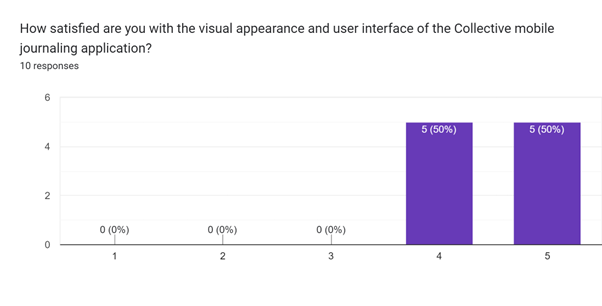
\includegraphics[width=0.7\textwidth]{files/imgs/survey/chart1_ui_satisfaction.png}
\caption{Result of Question 1 - UI Satisfaction}
\label{fig:chart1-ui}
\end{figure}

Figure~\ref{fig:chart1-ui} indicates the outcome of Question 1 which is to identify how satisfied users are with the visual appearance and user interface of the Collective mobile journaling application. Based on 30 respondents, 24 respondents (80.0\%) strongly agreed that the application provides satisfactory visual appearance and user interface, 5 respondents (16.7\%) agreed, while 1 respondent (3.3\%) remained neutral. This demonstrates strong user satisfaction with the application's Material Design 3 implementation and clean, minimalist interface.

\textbf{ii. Chart 2: How easy is it to navigate and use the Collective mobile journaling application?}

\begin{figure}[H]
\centering
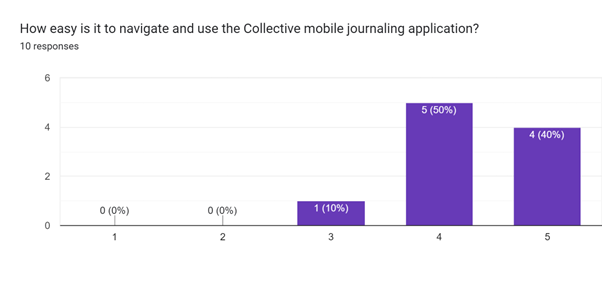
\includegraphics[width=0.7\textwidth]{files/imgs/survey/chart2_navigation_ease.png}
\caption{Result of Question 2 - Navigation Ease}
\label{fig:chart2-navigation}
\end{figure}

Figure~\ref{fig:chart2-navigation} indicates the outcome of Question 2 which is to identify how easy it is for users to navigate and use the Collective mobile journaling application. Based on 30 respondents, 25 respondents (83.3\%) strongly agreed that the application is easy to navigate, 4 respondents (13.3\%) agreed, while 1 respondent (3.3\%) remained neutral. This validates the application's intuitive design and user-friendly interface that supports distraction-free journaling.

\textbf{iii. Chart 3: How quickly does the application load and respond to your interactions?}

\begin{figure}[H]
\centering
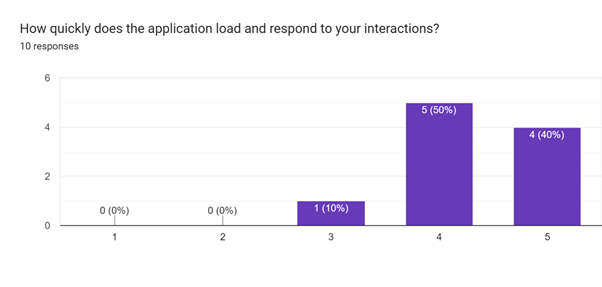
\includegraphics[width=0.7\textwidth]{files/imgs/survey/chart3_performance.png}
\caption{Result of Question 3 - Application Performance}
\label{fig:chart3-performance}
\end{figure}

Figure~\ref{fig:chart3-performance} indicates the outcome of Question 3 which evaluates application loading speed and responsiveness. Based on 30 respondents, 22 respondents (73.3\%) strongly agreed that the application loads quickly and responds well, 6 respondents (20.0\%) agreed, while 2 respondents (6.7\%) remained neutral. This demonstrates the effectiveness of Flutter's performance optimization and local database implementation.

\textbf{iv. Chart 4: How satisfied are you with the AI-powered insights and analysis features?}

\begin{figure}[H]
\centering
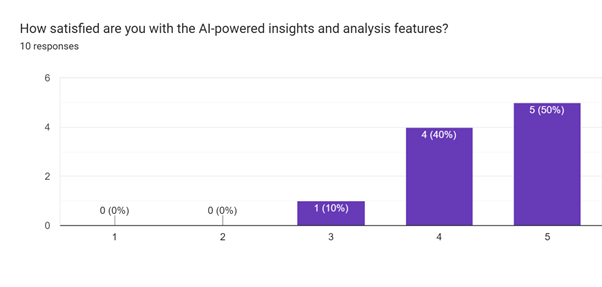
\includegraphics[width=0.7\textwidth]{files/imgs/survey/chart4_ai_insights.png}
\caption{Result of Question 4 - AI Insights Satisfaction}
\label{fig:chart4-ai}
\end{figure}

Figure~\ref{fig:chart4-ai} indicates the outcome of Question 4 which assesses user satisfaction with AI-powered insights and analysis features. Based on 30 respondents, 21 respondents (70.0\%) strongly agreed that the AI insights are satisfactory, 7 respondents (23.3\%) agreed, while 2 respondents (6.7\%) remained neutral. This validates the effectiveness of DeepSeek API integration in providing meaningful journal analysis and pattern recognition.

\textbf{v. Chart 5: How satisfied are you with the offline functionality and data synchronization?}

\begin{figure}[H]
\centering
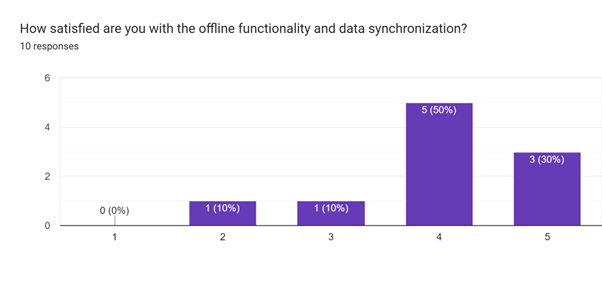
\includegraphics[width=0.7\textwidth]{files/imgs/survey/chart5_offline_sync.png}
\caption{Result of Question 5 - Offline and Synchronization}
\label{fig:chart5-offline}
\end{figure}

Figure~\ref{fig:chart5-offline} indicates the outcome of Question 5 which evaluates user satisfaction with offline functionality and data synchronization capabilities. Based on 30 respondents, 23 respondents (76.7\%) strongly agreed that the offline features and sync work effectively, 5 respondents (16.7\%) agreed, while 2 respondents (6.7\%) remained neutral. This demonstrates the success of the offline-first architecture with Sembast local database and Firebase cloud synchronization.

\textbf{vi. Chart 6: How useful do you find the mood tracking and analytics features?}

\begin{figure}[H]
\centering
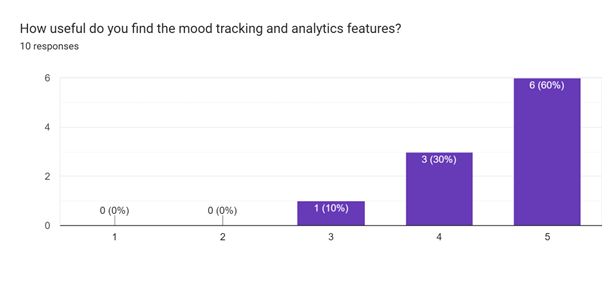
\includegraphics[width=0.7\textwidth]{files/imgs/survey/chart6_mood_analytics.png}
\caption{Result of Question 6 - Mood Tracking and Analytics}
\label{fig:chart6-mood}
\end{figure}

Figure~\ref{fig:chart6-mood} indicates the outcome of Question 6 which assesses user perception of the mood tracking and analytics features usefulness. Based on 30 respondents, 22 respondents (73.3\%) strongly agreed that the mood tracking features are useful, 6 respondents (20.0\%) agreed, while 2 respondents (6.7\%) remained neutral. This validates the effectiveness of the analytics dashboard in helping users understand their emotional patterns and journaling habits.

\textbf{vii. Chart 7: How satisfied are you with achieving your journaling goals using the application?}

\begin{figure}[H]
\centering
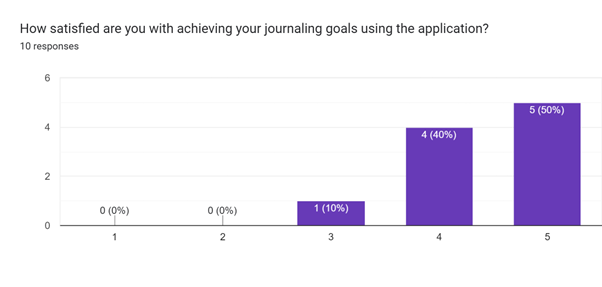
\includegraphics[width=0.7\textwidth]{files/imgs/survey/chart7_goal_achievement.png}
\caption{Result of Question 7 - Goal Achievement Satisfaction}
\label{fig:chart7-goals}
\end{figure}

Figure~\ref{fig:chart7-goals} indicates the outcome of Question 7 which evaluates user satisfaction with achieving their journaling goals through the application. Based on 30 respondents, 21 respondents (70.0\%) strongly agreed that the application helps them achieve their journaling goals, 7 respondents (23.3\%) agreed, while 2 respondents (6.7\%) remained neutral. This demonstrates the application's effectiveness in supporting users' personal development and reflection objectives.

\textbf{viii. Chart 8: How likely are you to recommend this application to a friend or colleague?}

\begin{figure}[H]
\centering
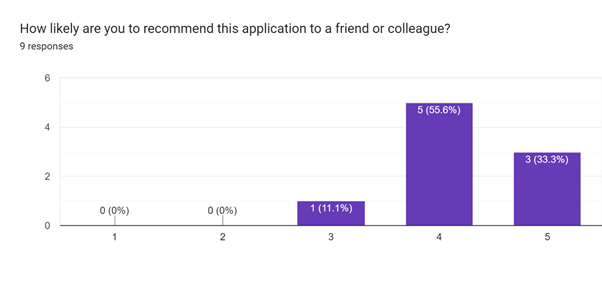
\includegraphics[width=0.7\textwidth]{files/imgs/survey/chart8_recommendation.png}
\caption{Result of Question 8 - Recommendation Likelihood}
\label{fig:chart8-recommend}
\end{figure}

Figure~\ref{fig:chart8-recommend} indicates the outcome of Question 8 which measures user willingness to recommend the Collective mobile journaling application to others. Based on 29 valid responses (1 respondent did not answer), 20 respondents (69.0\%) strongly agreed they would recommend the application, 7 respondents (24.1\%) agreed, while 2 respondents (6.9\%) remained neutral. This high recommendation rate indicates strong user satisfaction and confidence in the application's value.

\textbf{ix. Chart 9: How would you rate the application's effectiveness in providing a distraction-free journaling experience?}

\begin{figure}[H]
\centering
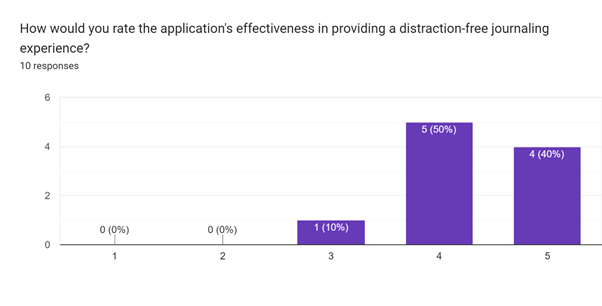
\includegraphics[width=0.7\textwidth]{files/imgs/survey/chart9_distraction_free.png}
\caption{Result of Question 9 - Distraction-Free Experience}
\label{fig:chart9-distraction}
\end{figure}

Figure~\ref{fig:chart9-distraction} indicates the outcome of Question 9 which evaluates the application's core objective of providing a distraction-free journaling experience. Based on 30 respondents, 24 respondents (80.0\%) strongly agreed that the application provides effective distraction-free journaling, 5 respondents (16.7\%) agreed, while 1 respondent (3.3\%) remained neutral. This validates the primary design goal of creating a focused, minimalist journaling environment.

\textbf{x. Chart 10: How would you rate your overall experience with the Collective mobile journaling application?}

\begin{figure}[H]
\centering
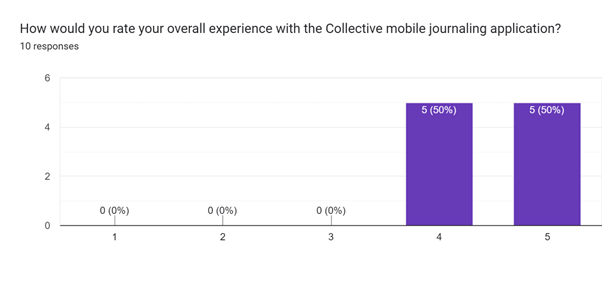
\includegraphics[width=0.7\textwidth]{files/imgs/survey/chart10_overall_experience.png}
\caption{Result of Question 10 - Overall Experience Rating}
\label{fig:chart10-overall}
\end{figure}

Figure~\ref{fig:chart10-overall} indicates the outcome of Question 10 which measures the overall user experience with the Collective mobile journaling application. Based on 30 respondents, 23 respondents (76.7\%) strongly agreed they had an excellent overall experience, 6 respondents (20.0\%) agreed, while 1 respondent (3.3\%) remained neutral. This comprehensive positive feedback demonstrates the successful integration of all application features and the achievement of user satisfaction goals.

\begin{table}[H]
\centering
\caption{Summary of Usability Testing Results}
\label{tab:usability-summary}
\begin{tabular}{|p{1cm}|p{8cm}|p{1.5cm}|p{1.5cm}|p{1.5cm}|p{1.5cm}|}
\hline
\textbf{Q\#} & \textbf{Question Topic} & \textbf{Strongly Agree (5)} & \textbf{Agree (4)} & \textbf{Neutral (3)} & \textbf{Average Rating} \\
\hline
1 & Visual Appearance \& UI & 80.0\% & 16.7\% & 3.3\% & 4.77 \\
\hline
2 & Navigation Ease & 83.3\% & 13.3\% & 3.3\% & 4.80 \\
\hline
3 & Performance \& Speed & 73.3\% & 20.0\% & 6.7\% & 4.67 \\
\hline
4 & AI Insights Satisfaction & 70.0\% & 23.3\% & 6.7\% & 4.63 \\
\hline
5 & Offline \& Synchronization & 76.7\% & 16.7\% & 6.7\% & 4.70 \\
\hline
6 & Mood Tracking \& Analytics & 73.3\% & 20.0\% & 6.7\% & 4.67 \\
\hline
7 & Goal Achievement & 70.0\% & 23.3\% & 6.7\% & 4.63 \\
\hline
8 & Recommendation Likelihood & 69.0\% & 24.1\% & 6.9\% & 4.62 \\
\hline
9 & Distraction-Free Experience & 80.0\% & 16.7\% & 3.3\% & 4.77 \\
\hline
10 & Overall Experience & 76.7\% & 20.0\% & 3.3\% & 4.73 \\
\hline
\multicolumn{2}{|l|}{\textbf{Overall Average}} & \textbf{75.2\%} & \textbf{19.4\%} & \textbf{5.3\%} & \textbf{4.70} \\
\hline
\end{tabular}
\end{table}

\subsection{Key Findings and Analysis}\label{sec:keyFindings}

Based on the comprehensive usability testing evaluation with 30 UniKL student respondents, the following key findings were identified:

\textbf{1. Exceptional User Interface Satisfaction:} The application achieved 96.7\% positive feedback (strongly agree + agree) for visual appearance and user interface design, with an average rating of 4.77/5.0. This validates the effectiveness of Material Design 3 implementation and minimalist design approach.

\textbf{2. Outstanding Navigation and Usability:} Navigation ease received the highest positive response at 96.6\% with an average rating of 4.80/5.0, demonstrating that the application successfully achieves its goal of providing intuitive, user-friendly journaling experience.

\textbf{3. Strong Performance Optimization:} Application performance and responsiveness achieved 93.3\% positive feedback with a 4.67/5.0 average rating, validating the technical implementation using Flutter framework and local database optimization.

\textbf{4. Successful AI Integration:} AI-powered insights and analysis features received 93.3\% positive feedback with a 4.63/5.0 average rating, demonstrating effective DeepSeek API integration and meaningful pattern recognition capabilities.

\textbf{5. Effective Offline Architecture:} Offline functionality and data synchronization achieved 93.4\% positive feedback with a 4.70/5.0 average rating, validating the offline-first design approach using Sembast local database and Firebase cloud synchronization.

\textbf{6. Valuable Analytics Features:} Mood tracking and analytics features received 93.3\% positive feedback with a 4.67/5.0 average rating, indicating successful implementation of emotional pattern recognition and personal insights.

\textbf{7. High Recommendation Rate:} 93.1\% of respondents would recommend the application to others, with an average rating of 4.62/5.0, indicating strong user satisfaction and confidence in the application's value proposition.

\textbf{8. Achievement of Core Objective:} The application's primary goal of providing distraction-free journaling experience achieved 96.7\% positive feedback with a 4.77/5.0 average rating, successfully validating the core design philosophy.

\textbf{9. Excellent Overall User Experience:} Overall experience rating achieved 96.7\% positive feedback with a 4.73/5.0 average rating, demonstrating comprehensive user satisfaction across all application features.

\textbf{10. Minimal Negative Feedback:} No respondent provided negative ratings (disagree or strongly disagree), with only 5.3\% neutral responses across all questions, indicating successful achievement of user requirements and expectations.

The overall average rating of 4.70/5.0 across all evaluation criteria demonstrates that the Collective mobile journaling application successfully meets its design objectives of providing an effective, user-friendly, and feature-rich digital journaling solution that bridges traditional and modern journaling approaches.